\documentclass[UTF8,oneside]{pkuthss}
\usepackage[backend = biber, style = gb7714-2015ay, url=false,gbtitlelink=true]{biblatex}
\usepackage{longtable}
\usepackage{multirow}
\usepackage{booktabs}
\usepackage{float}
\usepackage{caption}
\renewcommand*{\bibfont}{\zihao{5}\linespread{1.27}\selectfont}
\setlength{\bibitemsep}{3bp}
\newif\ifblind\blindfalse
\pkuthssinfo{
	cthesisname = {学士学位论文}, ethesisname = {Bachelor Thesis},
	thesiscover = {本科学位论文},
	ctitle = {我国债券市场违约特征分析},
	etitle = {Why Company Fails: A Bond Market View},
	cauthor = {董晨阳}, eauthor = {Ernest Dong}, date = {\today},
	studentid = {1800015446}, school = {经济学院},
	cmajor = {保险学}, emajor = {Risk Management and Insurance},
	direction = {}, mentorlines = {1},
	cmentor = {刘新立},
	ementor = {Xinli Liu},
	ckeywords = {信用风险,违约},
	ekeywords = {Credit Risk, Default},
}
\addbibresource{thesis.bib}
\newtheorem{hyp}{H}
\begin{document}
\frontmatter
\pagestyle{empty}
\maketitle
\clearpage
%!TEX root = ../thesis.tex
% Copyright (c) 2008-2009 solvethis
% Copyright (c) 2010-2017,2021 Casper Ti. Vector
% All rights reserved.
%
% Redistribution and use in source and binary forms, with or without
% modification, are permitted provided that the following conditions are
% met:
%
% * Redistributions of source code must retain the above copyright notice,
%   this list of conditions and the following disclaimer.
% * Redistributions in binary form must reproduce the above copyright
%   notice, this list of conditions and the following disclaimer in the
%   documentation and/or other materials provided with the distribution.
% * Neither the name of Peking University nor the names of its contributors
%   may be used to endorse or promote products derived from this software
%   without specific prior written permission.
%
% THIS SOFTWARE IS PROVIDED BY THE COPYRIGHT HOLDERS AND CONTRIBUTORS "AS
% IS" AND ANY EXPRESS OR IMPLIED WARRANTIES, INCLUDING, BUT NOT LIMITED TO,
% THE IMPLIED WARRANTIES OF MERCHANTABILITY AND FITNESS FOR A PARTICULAR
% PURPOSE ARE DISCLAIMED. IN NO EVENT SHALL THE COPYRIGHT HOLDER OR
% CONTRIBUTORS BE LIABLE FOR ANY DIRECT, INDIRECT, INCIDENTAL, SPECIAL,
% EXEMPLARY, OR CONSEQUENTIAL DAMAGES (INCLUDING, BUT NOT LIMITED TO,
% PROCUREMENT OF SUBSTITUTE GOODS OR SERVICES; LOSS OF USE, DATA, OR
% PROFITS; OR BUSINESS INTERRUPTION) HOWEVER CAUSED AND ON ANY THEORY OF
% LIABILITY, WHETHER IN CONTRACT, STRICT LIABILITY, OR TORT (INCLUDING
% NEGLIGENCE OR OTHERWISE) ARISING IN ANY WAY OUT OF THE USE OF THIS
% SOFTWARE, EVEN IF ADVISED OF THE POSSIBILITY OF SUCH DAMAGE.

% 此处不用 \specialchap,因为学校要求目录不包括其自己及其之前的内容。
\chapter*{版权声明}
% 综合学校的书面要求及 Word 模版来看,版权声明页不用加页眉、页脚。
\thispagestyle{empty}

任何收存和保管本论文各种版本的单位和个人,
未经本论文作者同意,不得将本论文转借他人,
亦不得随意复制、抄录、拍照或以任何方式传播。
否则,引起有碍作者著作权之问题,将可能承担法律责任。

% 若须排版二维码,请将二维码图片重命名为“barcode”,
% 转为合适的图片格式,并放在当前目录下,然后去掉下面 2 行的注释。
%\vfill\noindent
%\includegraphics[height = 5em]{barcode}

% vim:ts=4:sw=4

\begin{table}[h]
	\centering
	\begin{tabular}{|p{0.2\linewidth}p{0.2\linewidth}p{0.2\linewidth}p{0.2\linewidth}|}
		\hline
		\multicolumn{4}{|c|}{\large\textbf{本科学生毕业论文指导教师成绩评定表}}                                                      \\
		\multicolumn{4}{|c|}{}                                                                                        \\
		\hline
		\multicolumn{1}{|l|}{}         & \multicolumn{1}{|l|}{} & \multicolumn{1}{|l|}{}              & \multicolumn{1}{|l|}{} \\
		\multicolumn{1}{|l|}{学生姓名} & \multicolumn{1}{|l|}{董晨阳} & \multicolumn{1}{|l|}{学号}          & \multicolumn{1}{|l|}{1800015446} \\
		\multicolumn{1}{|l|}{}         & \multicolumn{1}{|l|}{} & \multicolumn{1}{|l|}{}              & \multicolumn{1}{|l|}{} \\
		\hline
		\multicolumn{1}{|l|}{}         &                        &                                     &                        \\
		\multicolumn{1}{|l|}{论文题目} &  \multicolumn{3}{|l|}{我国债券市场违约特征分析}                        \\
		\multicolumn{1}{|l|}{}         &                        &                                     &                        \\
		\hline
		\multicolumn{4}{|l|}{}                                                                                                 \\
		\multicolumn{4}{|l|}{指导教师评阅意见:}                                                                               \\
		\multicolumn{4}{|l|}{}                                                                                                 \\
		\multicolumn{4}{|l|}{}                                                                                                 \\
      \multicolumn{4}{|l|}{
      \qquad 债券违约受到多方面因素的影响,如何从全面视角出发对债券违约特征

      }\\
      \multicolumn{4}{|l|}{
      进行综合评价,对于债券违约的预警等具有重要意义。论文《我国债券市场违

      }\\
      \multicolumn{4}{|l|}{
      约特征分析》以此为出发点,基于大量相关数据,进行了实证研究。本文研究

      }\\
      \multicolumn{4}{|l|}{
      方法得当,结构清晰、重点突出,逻辑严密,引用资料准确、丰富,结论正确,

      }\\
      \multicolumn{4}{|l|}{
      文中用语和图表格式等符合本科论文的要求。作者在前人研究的基础上,从宏

      }\\
      \multicolumn{4}{|l|}{
      观、中观和微观三个层面出发选取指标、构建模型,对债券违约进行综合评价,

      }\\
      \multicolumn{4}{|l|}{
      并通过计量及机器学习方法进行了定量分析,具有一定的创新性,反映出该生

      }\\
      \multicolumn{4}{|l|}{
      对此问题经过了深入的思考,具有一定的研究能力,论文达到本科论文的要求。}\\
		\multicolumn{4}{|l|}{}                                                                                                 \\
		\multicolumn{4}{|l|}{}                                                                                                 \\
		\multicolumn{4}{|l|}{}                                                                                                 \\
		\multicolumn{4}{|l|}{}                                                                                                 \\
		\multicolumn{4}{|l|}{}                                                                                                 \\
		\multicolumn{4}{|l|}{}                                                                                                 \\
		\multicolumn{4}{|l|}{}                                                                                                 \\
		\multicolumn{4}{|l|}{}                                                                                                 \\
		\multicolumn{4}{|l|}{}                                                                                                 \\
		\multicolumn{4}{|l|}{}                                                                                                 \\
		\multicolumn{4}{|l|}{}                                                                                                 \\
		\multicolumn{4}{|l|}{}                                                                                                 \\
		\multicolumn{4}{|l|}{}                                                                                                 \\
		\multicolumn{4}{|l|}{}                                                                                                 \\
		\hline
		\multicolumn{4}{|l|}{}                                                                                                 \\
		\multicolumn{4}{|l|}{指导教师建议论文成绩为:}                                                                         \\
		\multicolumn{4}{|l|}{}                                                                                                 \\
		                               &                        & \multicolumn{2}{l|}{指导教师签名:}                          \\
		                               &                        & \multicolumn{2}{l|}{日期:}                                    \\
		\multicolumn{4}{|l|}{}                                                                                                 \\
		\hline
	\end{tabular}
\end{table}

\clearpage
\pagestyle{plain}
\setcounter{page}{0}
\pagenumbering{Roman}
%!TEX root = ../thesis.tex
\begin{cabstract}
	偶发的债券违约是经济体排除不稳定因素、自发降低系统性风险的正常现象,维持“刚兑”的债券市场反而是不健康的。但违约结果造成的影响是多方面的,处理得当可以使短期遭受困难的企业焕发新生,处理不当则可能影响金融市场稳定,进而对实体经济造成巨大影响。
	本文从债券违约的影响因素出发,以2014年来债券发行数据为样本,对我国债券市场上违约发行人的共性特征进行了分析,抽离出导致企业违约的重要因素,并通过机器学习的方式佐证和拓展了计量模型,以期对债券市场违约有一个比较好的刻画。研究发现:企业的经营收入、财务效率与宏观经济的波动率对企业债券违约有显著影响。
\end{cabstract}
\begin{eabstract}
	Occasional bond default is a normal phenomenon for an economy to eliminate unstable factors and spontaneously reduce systemic risks. It is unhealthy to maintain a bail out bond market. However, the impact of the default results is multi-faceted. Proper handling can rejuvenate companies that have suffered short-term difficulties. Improper handling may affect the stability of the financial market, and thus have a huge impact on the real economy.
	Starting from the influencing factors of bond defaults and taking the bond issuance data since 2014 as a sample, this paper analyzes the common characteristics of default issuers in Chinese bond market, extracts important factors that lead to corporate defaults, and uses machine learning. And extended the econometric model in order to have a better characterization of the bond market default. The study found that: the operating income, financial efficiency and macroeconomic volatility of enterprises have a significant impact on corporate bond defaults.
\end{eabstract}

\tableofcontents
\mainmatter
%!TEX root = ../thesis.tex

\chapter{引言}

\section{我国信用债违约回顾}

过去一段时间,我国信用债市场维持着“刚兑”神话,而自 2014 年“11 超日债”违约以来,我国信用债市场中投资者“刚性兑付”的“信仰”逐步动摇、破灭。及至 2021 年,永城煤电、华晨宝马的违约打破了人们对 AAA 级国企的“刚兑信仰”,恒大、海航违约使人们意识到并不存在所谓“大而不倒”。近年来一些典型的债券违约事件如表\ref{tab:defaults_in_history}所示。

\begin{table}[ht]
	\caption{近年来部分影响较大的违约事件}
	\centering
	\begin{tabular}{lccc}
		债券名称         & 违约日期   & 原因               & 影响                   \\ \hline
		11超日债         & 2014-03-05 & 过度扩张资金链断裂 & 打破刚兑的开始         \\
		11天威MTN2       & 2015-04-21 & 经营亏损资不抵债   & 打破国企刚兑           \\
		14波鸿CP001      & 2015-04-12 & “技术性”违约       & 首例“技术性违约”       \\
		15五洋债         & 2018-08-16 & 欺诈发行           & 首例公司债券欺诈发行案 \\
		16民生投资PPN001 & 2019-01-29 & “技术性”违约       & AAA 债券违约第一例     \\
		20永煤SCP003     & 2020-11-26 & 逃废债             & 河南全省融资环境恶化   \\
		15天安人寿       & 2020-12-29 & 股东抽血           & 金融机构破刚兑付       \\
		17幸福基业MTN001 & 2021-02-27 & 过度扩张遇宏观调控 & 地产债违约潮的开始     \\
	\end{tabular}
	\label{tab:defaults_in_history}
\end{table}
事实上,“刚兑”并非正常现象,反而容易导致风险的无序累积。在经济周期的起伏过程中,企业经营失败不可避免。通过违约释放部分信用风险,反而能降低大规模系统性金融风险发生的概率。违约可以使泡沫膨胀到更大前提前破裂,如近期的房地产企业的加速出清,就是过去房企高杠杆经营扩张的反噬。如果长时间维持高杠杆经营,居民部门负债率高企,地产商开发贷终将难以维续,势必会对银行系统造成很大的威胁,进而影响我国金融稳定。

然而,债务违约毕竟会带来多方面的危害。对投资人来说,投资失败意味着不小的损失;对发行人则意味着丧失外部融资功能、经营难以维系。此外,违约还有一定的外部性,如果处理不好,如永煤逃废债,则可能会影响区域乃至全国的投融资环境,进而会对整个经济体造成影响。这些企业违约的原因各有不同,主要包括:技术原因场外兑付(如中融新大),评级公司下调评级(如花样年、新力),公司流动性遇到了暂时的困难(如恒大)等。因此,如何准确评估企业违约风险,使得各方利益相关者在违约事件出现之前有所准备,是一个重要问题。

\begin{figure}[ht]
	\centering
	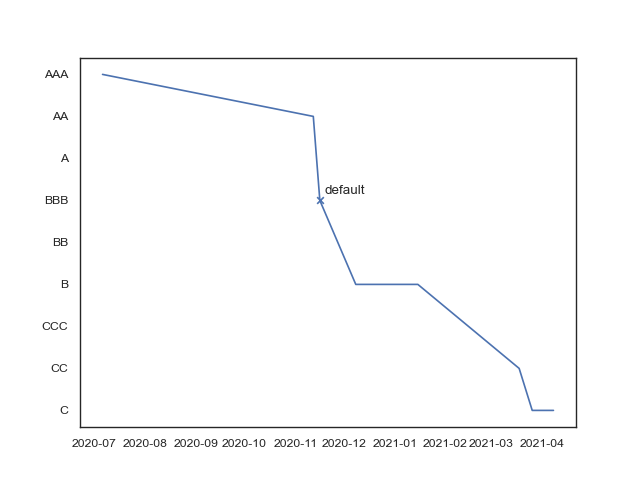
\includegraphics[width=0.9\linewidth]{./data/rating_of_zg.png}
	\caption{某评级公司对某违约发行人的历史评级}
	\label{fig:rating_of_zg}
\end{figure}
评级是债券信用风险评估的常用工具,是判断公司违约风险最直观的手段,但信用评级却屡屡失灵。例如,有些评级机构为了维护发行人利益,初始时给予某债券很高的评级,随后在违约事件已经板上钉钉的情况下,几天内连续下调原先的虚高评级至垃圾级,如图\ref{fig:rating}所示的某违约企业评级历史。又如,被\Textcite{王雄元2013声誉机制}列为低声誉评级机构的大公国际,因涉嫌帮助欺诈发行“五洋债”,应承担 10\% 的连带责任赔偿 7400 万元。但大公竟称“公司已经发不出工资,顶多赔偿 150 万元”,最终被列入失信被执行人,可见某些评级机构对自身声誉的重视程度。因此,本文试图从微观、中观和宏观三个层面出发,对企业债券违约的影响因素进行分析,探讨对债券违约风险进行全面客观评价的模型。

本文主要内容如下:第一章回顾并梳理现有的有关研究;第二章基于理论和实践归纳违约的影响因素;第三章分别基于计量和机器学习手段进行了研究设计,第四章对理论进行实证检验,第五章进行了稳健性检验;第六章对全文进行总结。
\section{文献综述}
\label{sec:zs}
在信用评级质量方面,很多研究发现,评级机构的利益动机会对评级质量产生影响。评级机构在行业竞争的情况下,为了获得收入,会对公司虚高评级,即使是国际著名的评级机构也无法避免\cite{opp2013rating}。甚至在违约发生后,涉事评级机构非但不考虑模型是否有偏误,反而为了争取市场份额而放宽标准,以提高评级\cite{黄小琳2017债券违约对涉事信用评级机构的影响}。此外,付费模式也会使得评级机构失去独立性,在“发行人付费”模式下,信用评级虽然可以在一定程度上包含公司的内部私有信息,但由于独立性缺失,其总体的信用评级质量仍然低于“投资人付费”模式下的信用评级质量,使得部分评级机构声誉较差\cite{吴育辉2020,陈关亭2021多重信用评级与债券融资成本}。因此,评级可能并不是一种有效的信用评估方式 \cite{blochlinger2018ratings}。

除评级之外,学者们还从不同层面讨论了违约的影响因素。

在公司层面,对违约的讨论主要基于公司治理。\Textcite{林晚发2018高管任职经历的得与失}从高管任职经历出发,发现有高管担任过人大代表或政协委员的企业债券发行成功率更高,\Textcite{anginer2018corporate}提出一个涵盖管理、约束、独立三方面指标的公司治理指标,并指出公司治理增加一个标准差使银行的违约距离指标降低了 0.14 个标准差。\Textcite{ding2021corporate}和\Textcite{subrahmanyam2017credit}分别从疫情和引入 CDS 对公司治理的影响出发, 研究外生冲击由于公司治理能力的差异影响偿债能力的差异。

在市场层面,有学者从市场信号的角度研究违约。有些是直接研究信用债的利差,如\Textcite{纪志宏2017信用风险溢价还是市场流动性溢价}利用跨市场债的利差分析流动性和信用风险分别对利差的贡献。也有些是利用信用衍生品的数据,如\Textcite{bonaccolto2021breakup}利用 CDS ,研究疫情对欧盟成员国债券违约风险的冲击。经典的信用风险模型如莫顿模型、KMV 模型等亦是利用市场价格信号预测违约的,但是这些理论在实践中系统性地低估了实际投资级债券信用利差的水平,即所谓“信用利差之谜”,\Textcite{feldhutter2018myth}认为源于莫顿模型的不正确应用,而\Textcite{bai2020credit}则持相反观点,认为是巨大的市场风险价格归因于具有重大下行尾部风险敞口的证券,标准的基于扩散的违约结构模型被错误指定,因而模型显著低估了短期信用利差。

在宏观层面,\Textcite{bai2019common} 和\Textcite{bali2021macroeconomic}分别从宏观经济下行和宏观经济不确定性出发,研究宏观环境对于公司债利差的影响。宏观政策角度,\Textcite{王博2019货币政策不确定性}指出货币政策不确定性的增加会带来违约风险的上升。\Textcite{梅冬州2021财政扩张} 和\Textcite{2020Fiscal} 则认为财政扩张导致挤出效应,从而民企面临融资困境,进而违约率上升,利差走阔。此外,流动性可能会影响违约\cite{brogaard2017stock},更高的流动性可以通过提高价格效率来降低违约风险,或者通过放松投资者的退出能力来改善公司治理。

在风险传染方面,有关研究主要集中在系统性风险传染。\Textcite{苟文均2016债务杠杆与系统性风险传染机制}基于 CCA 模型,提出杠杆率应从较高居民转移至政府等低杠杆部门,以降低违约风险。
\Textcite{2020Do}基于 VaR 模型,认为几乎所有的系统性风险指标对对违约率都有预测能力。
非系统性风险方面,\Textcite{azizpour2018exploring}认为公司之间的财务、法律或业务关系可能充当风险分散的渠道,通过捕捉系统性风险和这种非系统性的聚类,可以几乎完美地匹配了的时间变化结果所隐含的时间变化的违约计数和违约时间的理论分布。

综上,现有文献较为分散地分析单方面影响违约的因素,少有揭示违约因素间的相互作用,且对我国目前债券市场上风险逐步释放的现状估计不足。因此,本文聚焦于将不同违约因素进行整合,采用自下而上的方式,归纳违约因素,比较违约因素之间的相对重要性,并通过决策树、随机森林等算法刻画违约因素之间的相互作用。
本文的贡献在于:结合理论与实务中的新现象,系统性整理了违约因素,并采用机器学习算法探究违约因素间的相互作用。

%!TEX root = ../thesis.tex

\chapter{理论模型}
综合 \ref{sec:zs} 中各学者的观点,以及现实中的违约案例,本文将从宏观、中观以及微观角度,拆解可能影响违约的因素。
\section{微观层次}
本文将微观层面影响企业违约的因素分为以下四类,主要包含企业级的指标:
\subsection{公司层面}

国企发行了80\%的债券,但违约中只占了15\%,有学者指出可能是由于国企存在政府支持\cite{mo2021china},也有可能国企通常相对资金雄厚,经营情况较好。因此,本文将公司性质作为影响因素之一建模。
同样的,上市企业比非上市企业融资方式更多,融资额往往也更大,部分违约企业也将自我总结违约原因是上市失败,因此上市与否或许也可能影响违约。

股东对企业的支持也可能影响是否违约,如苏宁易购缺乏实控人,在企业危难时各股东自扫门前雪,没有人向企业注血,最终苏宁走向违约。通常而言大股东持股比例越高,对企业的重视程度会越大,更有可能为了避免违约后其持有的大量股权价值归零而为企业提供资金支持或豁免债务。

此外,正如\ref{sec:zs}中众多学者对公司治理的研究所揭示,公司治理成效也可能是影响违约因素。
但是一方面公司治理会影响违约与否,另一方面违约企业通常会面临法律纠纷、债权人接管等情况,令企业公司治理发生很大变化。本文计划以持有基金占比作为公司治理的代理变量。
公募基金虽然会考虑违约与否,但更加担心债券持有期间贬值。
公募基金持有债券类似于交易性金融资产,买入的目的可以是获得利息收入或者未来得到债券估值的资本利得;而银行持有债券交易更少,等待还本付息,类似于持有至到期投资。
公募基金在评级下调超出风控阈值后必须斩仓,即便债券因流动性过低有价无市,而所有违约债券都或迟或早会被下调为垃圾级,但评级下调的债券中违约中终究只是少数,因此公募基金持有比例与违约弱相关。
公募基金更多是扮演财务投资者的角色由于担心债券在持有期间贬值,这就使他们更加会担心企业公司治理存在问题。如果公司治理水平低,债券潜在的下跌可能性更大\Parencite{anginer2018corporate}。即基金持有比例和公司治理强相关。
因此本文计划采用基金持有比例来表征公司治理。

最后,公司层面还有一些难以量化到因素,如发行人主观意愿(花样年地产账面现金充足“花式”躺平违约)、财务造假(康美药业、五洋建设)。但因此违约的终是少数,绝大多数地产商苦苦挣扎避免躺平,绝大多数企业报表准确。因此本文不将这些因素纳入考虑。
\subsection{经营层面}
企业面临流动性危机,很多情况下是经营不及预期,营收大幅亏损,如原超日太阳在连续三年大额亏损后,最终无法兑付利息成为打破刚兑的第一例违约。

客户集中度过高,可能会导致企业面临较高的风险\cite{王雄元2017客户集中度与公司债二级市场信用利差}。集中的客户有能力要求企业降价、使用商票结算等以降低自身成本,通过压迫企业获得更大利润空间。例如建设承包商南通三建持有大量恒大商票得不到兑付,不得不寻求债务展期。

经营过程中的杠杆率也有可能影响违约\cite{王永钦2019杠杆率如何影响资产价格},如以“高杠杆-高周转”著称的恒大,在融资受限时高杠杆的游戏进行不下去。但一方面很多违约公司会美化负债率,用诸如战略投资者等明股实债的方式,用尽各种手段将负债隐藏到表外;另一方面,不同性质的行业杠杆差异较大,如重工业和服务业之间相似的负债率并不意味着相近的爆仓的可能性,简单的比较负债率并不可取。基于此本文不采用资产负债表科目刻画杠杆率,而是采用标准券折算率这一比较市场化的指标,即质押企业债券可以获得多大比例的标准券来衡量企业杠杆率。折算率高意味着市场允许企业可以通过质押债券的方式撬动更多融资,市场允许其加更高的杠杆。且折算率对于优质企业有上限,对于违约风险更大的企业更敏感。

\subsection{财务层面}
对于会计指标,\Textcite{blochlinger2018ratings}指出 Altman's Z 指标是一个比较综合的、很好的预测违约会计指标。
此外违约本质上是企业持有的现金及其等价物无法偿还到期债务,存在一定的可能公司真的遇到了短期流动性危机而未来长期表现将会王者归来,如盐湖股份短期流动性告急,通过银行债转股使其资产不至于低价贱卖流失,重整两年后成为锂矿龙头。因此本文也将考虑现金短债比这一因素。
\subsection{评级指标}
\ref{sec:zs} 中各学者对评级指标的批判非常有借鉴意义。但即便以预测的角度看评级并不完全准确,但以后验的角度看,评级也反映了一定的公开与非公开信息,因此本文也将主体评级纳入考虑。
\section{中观层次}
中观层次为非企业级、非全国级的因素。如行业、流动性和地理因素。

\begin{figure}[h]
	\centering
	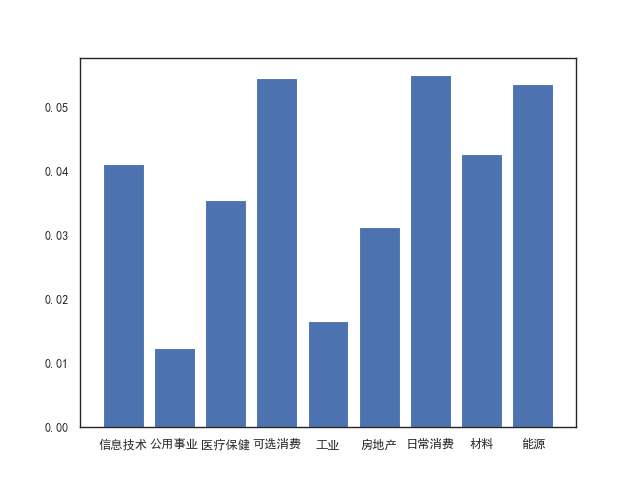
\includegraphics[width=.9\linewidth]{./data/industry.png}
	\caption{\label{fig:industry}违约债分行业分布}
\end{figure}

如表 \ref{fig:industry} 所示,看似较高违约率的行业,
均是因为单一主体违约余额较大(如方正集团导致计算机行业、华晨汽车导致汽车行业、紫光集团导致电子行业、山东如意导致纺织行业违约率激增)。如国外的情况\cite{azizpour2018exploring},我国债券违约亦基本可以排除大多数的行业聚类,即某行业因行业景气集中某段时间违约的情况。即便是近期的房地产违约风波,也并非主要由于行业景气度,而是由于房地产“三条红线”等政策约束高杠杆的经营。因此本文将主要考虑房地产政策(房地产行业且时间大于 2020 年),而不考虑每个行业本身。

\begin{figure}[h]
	\centering
	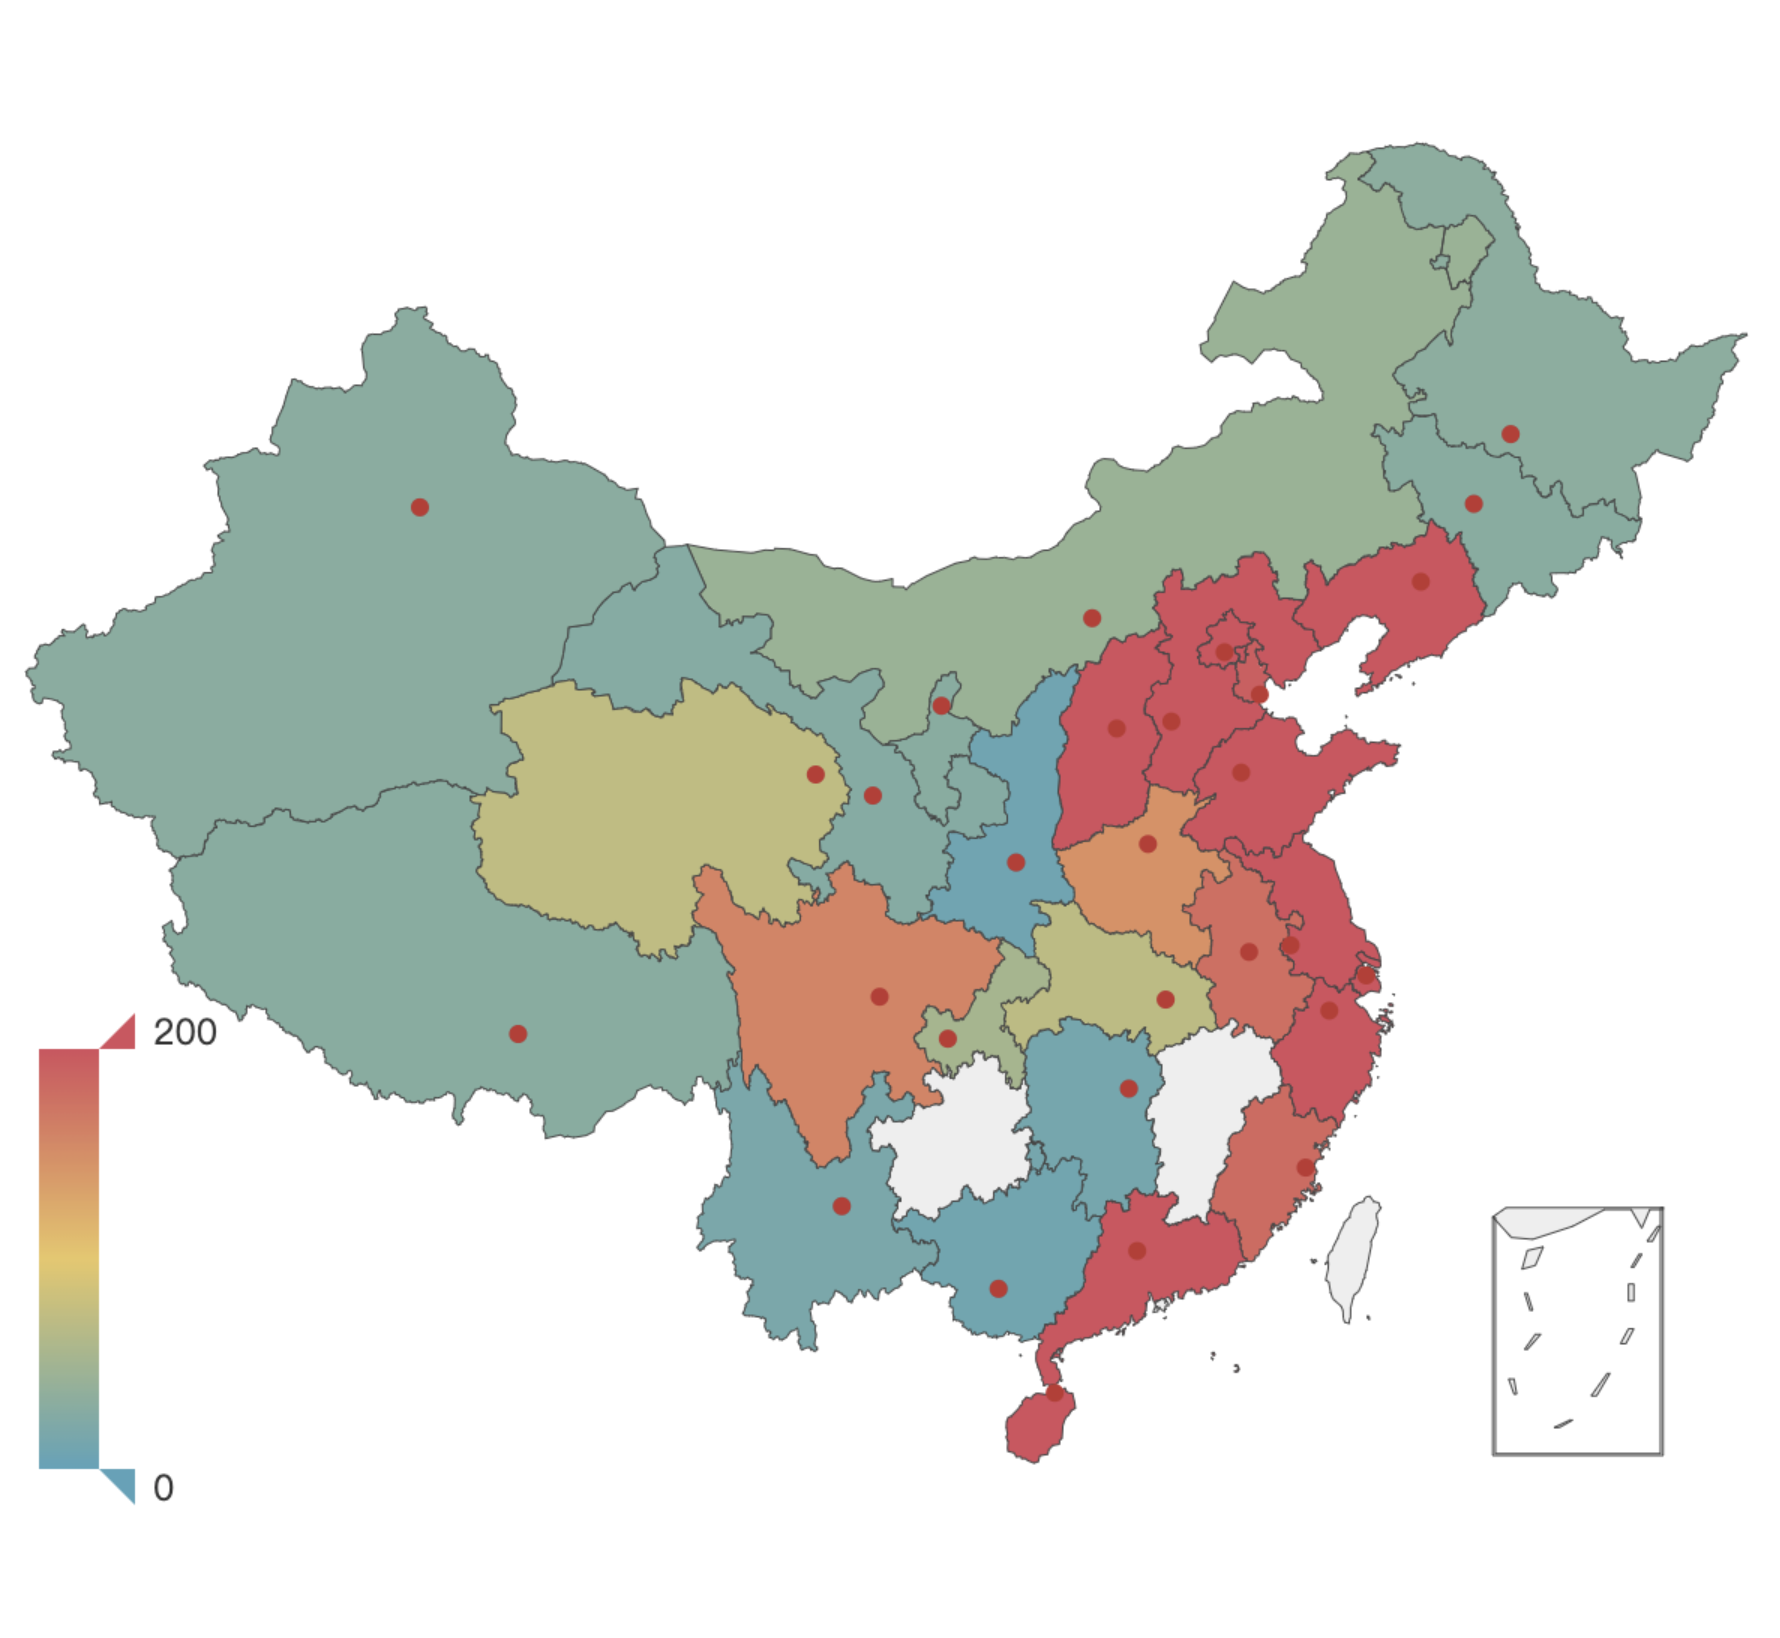
\includegraphics[width=.9\linewidth]{./data/default_by_geo.png}
	\caption{\label{fig:geo}违约债地理分布}
\end{figure}
地理上看,
一方面经济落后地区违约风险较大,一方面经济较好的地区企业发债数量较多可能导致违约金额较大,如图\ref{fig:geo}显示出后一种作用较强,尽管某些经济欠发达地区似乎仍然维持刚性兑付。尽管看似部分地区违约率高,但事实上高违约率的原因大多也是单一违约主体违约金额大,如河北的华夏幸福、辽宁的华晨宝马、海南的海航、青海的青国投等等,总的来说地理上的传染尚不明晰。

最后是流动性,本文计划以市场成交金额为流动性指标。当市场流动性偏紧时,如永煤违约后风险偏好迅速下降,各机构连 AAA 国企也不敢买,成交量萎靡流动性偏紧,进而导致一级市场上冀中能源、紫光、清华控股等无法发债接续,到期压力巨大,最终部分企业走向违约。
\section{宏观层次}
如\ref{sec:zs}中学者研究,货币政策与财政政策可能会对企业违约有影响。本文计划财政政策使用政府支出占GDP比重表征,货币政策以 SHIBOR 利率表征。

有学者对债券回报率做 Fama 因子分析
\cite{chung2019volatility}
,发现以 VIX 指数为代表的波动风险的影响是普遍存在的。
因此本文效仿选择上证 50 期权的隐含波动率作为波动率指标,2015 年期权推出之前则采用上证历史波动率。

%!TEX root = ../thesis.tex

\chapter{计量检验}
\section{数据清洗}
由于 2014 年以前有“刚兑神话”,企业无力负担债务时承销商、担保方或是股东会选择垫付以避免公开市场违约,因此我们选择的样本覆盖了 2014 年初至今发行的信用债发行人。考虑到我国金融机构和非金融机构之间存在很大的监管差异。金融机构特别是银行、保险等行业在出现风险时,往往由于涉及面众多,牵涉民生较广,可能会引发系统性风险,政府往往会及时采取手段控制风险,如接管安邦保险、包商银行、天安财险/人寿等金融机构。在真实的案例中,亦只有天安人寿一家有展期债券,其他保险公司和银行券商均没有违约。因此在建模过程中,我们会在数据中排除掉商业银行、保险公司、证券公司类的金融机构。

城投公司是我国一个独特的存在。截止 2022 年 2 月,我国信用债券市场中企业债、公司债、中期票据、短融、超短融以及定向工具存量 66.5 万亿,而城投债存量 13 万亿。
大多数区县级城投公司以及少数市级城投公司财务状况都很不健康:负债率居高不下,财政回款慢,公益性质大盈利能力不强。但迄今为止真正意义上的城投公司违约尚未出现。\Textcite{钟辉勇2016城投债的担保可信吗}就指出城投债可能存在隐性政府背书兜底。例如 2020 年底受永煤信用事件的冲击,投资者对违约的担忧上升、风险偏好下降,出现了“抱团”城投的现象。
2021 年 7 月银保监发 [2021]15 号文指出,各银行保险机构要严格执行地方政府融资相关政策要求,打消财政兜底幻觉,强化合规管理、尽职调查,不得以任何形式新增地方政府隐性债务。或许在将来城投公司违约将逐步正常化,但目前而言城投公司违约的影响因素尚不清晰且与其他企业区别较大,因此我们在数据中亦排除城投债。

不同评级公司的评级标准不同,划分的等级也有所不一。但大多评级都是分为 A、B、C 三档,每档中划分三个主要层次,最后辅以一个正负表示是否略高或略低于标准。在回归中我们将评级为最高 AAA 的划为一档,AA 及 A 划分为一档,BBB 以下至 B 以及 CCC 以下至 C 为一档。这么做的原因如 \ref{sec:zs} 中所述,我国评价公司评级比较扭曲,集中在 AAA 和 AA 。不同档次间违约概率差别不一定比较大,大量债券被划分为了高等级债券。为了降低评级不准确的影响,本文将评级按照上述标准分类。

最后,我们在回归中加入年份作为控制变量,以控制模型未关注到的事件冲击。

\section{计量回归分析}
清洗后 6412 家发行人符合条件,如表\ref{tab:Logitresult}所示为数据整理后 Logit 回归模型的部分结果。

%!TEX root = ../thesis.tex
\begin{table}
	\begin{center}
		\caption{Logit 模型回归结果\label{tab:Logitresult}}
		\begin{tabular}{lllll}
			\toprule
			                & Default I  & Default II & Default III & Default IIII \\
			\midrule
			\(Const\)       & -5.8949*** & -2.5416**  & -2.5158**   & -7.4246***   \\
			\(R_1\)         & 0.2259     & 0.1437     & 0.1731      & 0.1555       \\
			                & (0.6159)   & (0.7092)   & (0.7098)    & (0.7104)     \\
			\(R_2\)         & 3.9984***  & 3.3417***  & 3.3072***   & 3.2811***    \\
			                & (0.6581)   & (0.7559)   & (0.7516)    & (0.7535)     \\
			\(R_3\)         & 7.2459***  & 6.8585***  & 6.7762***   & 6.8656***    \\
			                & (0.6953)   & (0.7814)   & (0.7853)    & (0.7896)     \\
			\(Assets\)      &            & -0.0000    & -0.0000     & -0.0000      \\
			                &            & (0.0000)   & (0.0000)    & (0.0000)     \\
			\(Cash\)        &            & -0.5597    & -0.4909     & -0.4566      \\
			                &            & (0.4064)   & (0.4140)    & (0.4050)     \\
			\(Conversion\)  &            & -1.0608    & -1.0940     & -1.0416      \\
			                &            & (1.3674)   & (1.3246)    & (1.2942)     \\
			\(E_1\)         &            & -3.6293*** & -3.4614***  & -3.4205***   \\
			                &            & (0.7089)   & (0.7210)    & (0.7333)     \\
			\(E_2\)         &            & -2.9214*** & -3.0070***  & -2.9745***   \\
			                &            & (0.9253)   & (0.9274)    & (0.9370)     \\
			\(E_3\)         &            & -2.9634*** & -2.9664***  & -2.8548**    \\
			                &            & (1.0935)   & (1.1159)    & (1.1163)     \\
			\(Fund\)        &            & -0.2234*   & -0.1592     & -0.1532      \\
			                &            & (0.1296)   & (0.1394)    & (0.1353)     \\
			\(Income\)      &            & 0.0000     & 0.0000*     & 0.0000*      \\
			                &            & (0.0000)   & (0.0000)    & (0.0000)     \\
			\(Listed\)      &            & -0.5662    & -0.4617     & -0.5201      \\
			                &            & (0.3855)   & (0.3843)    & (0.3868)     \\
			\(Payable\)     &            & 0.0000     & -0.0000     & -0.0000      \\
			                &            & (0.0000)   & (0.0000)    & (0.0000)     \\
			\(Shareholder\) &            & -0.0019    & -0.0031     & -0.0037      \\
			                &            & (0.0054)   & (0.0054)    & (0.0054)     \\
			\(Z\)           &            & -0.0815*   & -0.0770*    & -0.0893**    \\
			                &            & (0.0432)   & (0.0427)    & (0.0447)     \\
			\(Estate\)      &            &            & 2.9755***   & 2.9305***    \\
			                &            &            & (0.9743)    & (0.9769)     \\
			\(Liquidity\)   &            &            & -0.0000     & -0.0000      \\
			                &            &            & (0.0000)    & (0.0000)     \\
			\(Fiscal\)      &            &            &             & 2.0446       \\
			                &            &            &             & (4.6763)     \\
			\(Monetary\)    &            &            &             & 0.5863       \\
			                &            &            &             & (0.4002)     \\
			\(Volatility\)  &            &            &             & 0.0670**     \\
			                &            &            &             & (0.0335)     \\
			\bottomrule
		\end{tabular}
	\end{center}
    \qquad \small{注:括号中为异方差稳健标准误下的 Z 值;***,**,*分别表示回归系数在1\%、5\%和10\%的水平上显著,下同。}
\end{table}

微观角度,评级 B/C 的企业,相较于评级 A以上企业违约率明显增加,而 AAA 企业相较于 AA 或 A 违约率差异不大,这是和预期相符的:A 评级及以上企业违约应是预期外事件,评级较低的企业更容易违约。

国企、外企、集体企业、民营企业违约可能性依次增加亦符合预期:国企可能存在一定的政府支持\autocite{mo2021china},而跨国企业通常资金雄厚。
2018-2019 年有过所谓的“民企违约潮”,这两年民企违约债券余额均超过1000亿元。背后原因有金融去杠杆造成的融资难,但究其本质还是由于边际上资质较差的民企在 2015 年发行公司债门槛降低后涌入债券市场,而资质较差国企在当时仍能获得满足其需要的银行贷款。

上市公司违约率较低但显著程度不高,亦启发我们通过一些资本运作尽管可以降低违约概率,但不违约终究还是需要坚实的基本面作为支撑。
违约本质上还是发行人可用的资金无法覆盖到期应付的债务,因此经营和财务指标对违约的解释力较强。主营收入的增多可以显著冲抵潜在违约的可能性,经营亏损则埋下了偿债能力不足的种子。财务指标 \(Z\) 值预警亦显著。

中观角度,房地产政策显著性很高。2020 年以来地产行业受到的冲击较大,企业融资受到约束,之前的高杠杆高周转的无序扩张的苦果使得地产债于 2021 年爆发了违约大潮,几乎所有的违约地产企业都是在 2021 年特别是后半年违约的。

宏观政策对违约显著性不高,这说明财政扩张导致“国进民退”是不成立的,而放松货币政策并非能降低违约率。财政扩张存在一定的挤出效应,但也存在一定的乘数效应,使企业收入提升进而影响违约率。放松货币政策的目的还是在于避免短时间内流动性收紧影响实体经济,而非在长期降低违约数量的发生。我国政策更多认为部分企业的违约是一种正常现象,但不希望大规模的集中违约,影响实体经济。
我国宏观政策很多是以稳为主的逆周期调节。因此大多数属逆周期的宏观政策对违约的解释力较低。
但是波动率显著,说明稳定的经济可以降低违约事件的发生,侧面显示出经济以稳为主的重要性。
\begin{figure}[h]
	\centering
	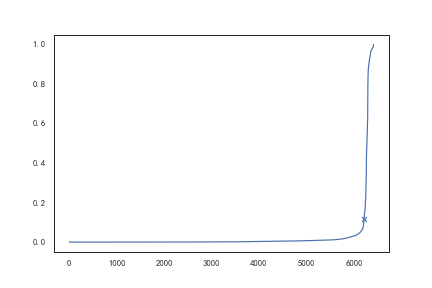
\includegraphics[width=0.9\linewidth]{./data/渤海银行.png}
	\caption{标记处为渤海租赁预测点}
	\label{fig:bhyh}
\end{figure}

\section{机器学习验证与比较}
违约实际上并非线性的因素叠加,包含了非线性的因素,如华夏幸福违约,既存在过度扩张导致现金流承压,又存在重要股东拒绝为其扩张买单,最终资金链断裂。虽然可以通过加入交互项刻画这种“同时发生”的作用,但会发生“维度灾难”,可用数据变得稀疏。
机器学习适合于提取其中非线性因素。但违约样本是偏态分布的,违约债只占约 1\%,通过神经网络等方式的机器学习极有可能会欠拟合或过拟合,使机器判断有误。
综合考虑下决定采用决策树和随机森林两种受样本分布偏态影响较小的方式进行预测。
决策树是通过二叉树这一数据结构,通过最大化信息增益的手段训练分类器,比较直观且可解释性较强。而随机森林则是一种集成算法,即通过构建多棵决策树“投票”的“森林”训练器,对于不平衡的数据集来说,它可以平衡误差,但缺乏可解释性。

决策树训练结果可视化如图\ref{fig:decision_tree}所示,Logit 模型和两种机器学习算法模型准确率如表\ref{tab:acc}所示。

\begin{figure}[h]
	\centering
	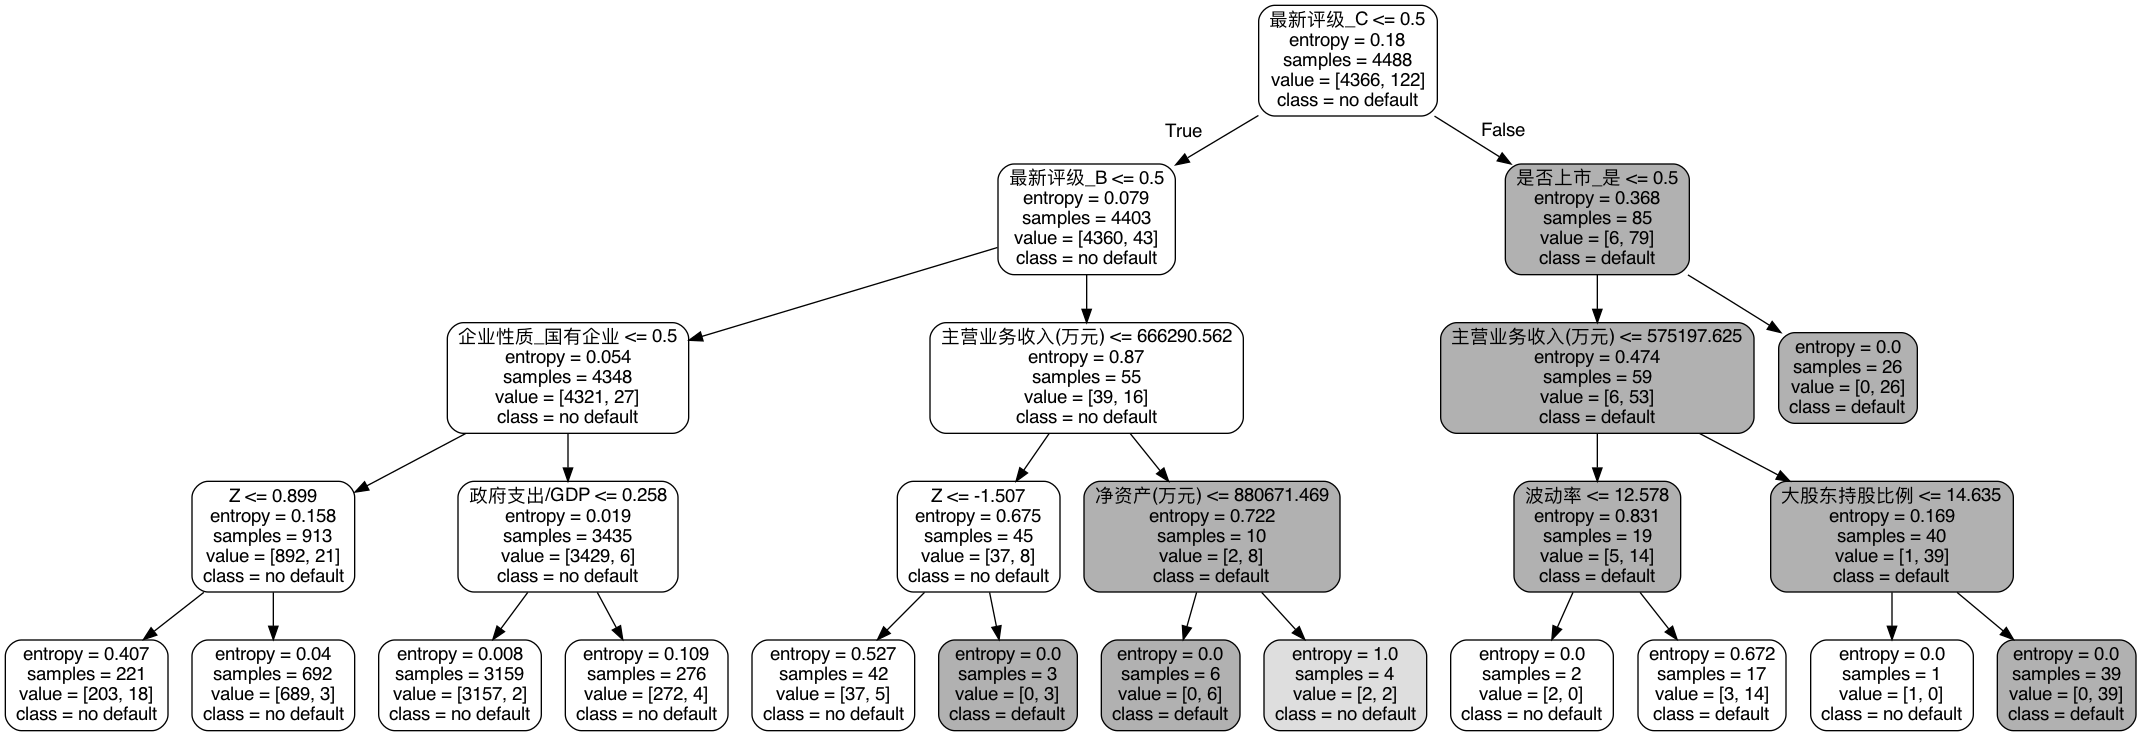
\includegraphics[width=.9\linewidth]{./data/decision_tree.png}
	\caption{\label{fig:decision_tree}决策树}
\end{figure}

图\ref{fig:decision_tree}决策树算法的关键节点如波动率、主营收入、企业性质、\(Z\) 值等在 Logit 模型中显著,在 Logit 模型中不显著的大股东持股比例分枝后判断的概率值仅勉强超过阈值,与 Logit 模型互相印证。

\begin{table}
	\caption{\label{tab:acc}不同模型的比较}
	\centering
	\begin{tabular}{lrrrrr}
		                      & accuracy & error rate & precision & recall & f1   \\
		\hline
		全部预测不违约        & 0.99     & 0.01       & -         & 0      & -    \\
		Logistic(全样本)      & 0.99     & 0.01       & 0.86      & 0.72   & 0.78 \\
		Decision Tree(测试集) & 0.99     & 0.01       & 0.93      & 0.73   & 0.82 \\
		Random Forest(测试集) & 0.99     & 0.01       & 0.85      & 0.70   & 0.76 \\
	\end{tabular}
\end{table}

表\ref{tab:acc}中准确率 accuracy 为预测正确的概率,精确率 precision 为预测违约的样本中确实违约的概率,召回率 recall 为事实违约样本中预测正确的概率。精确率和召回率是两个不同方面的分类器评价指标,他们的调和平均 F1 > 0.5 则说明该分类器是有效的。表\ref{tab:acc}中准确率与全部预测不违约的 0.99 相同,这是由于样本分布偏态造成的。但 F1 值均高于 0.5 ,证明本文使用的三个分类器都有一定的价值。且决策树算法相对优于其他算法。
决策树优于 Logit 模型算法在于其包含了非线形因素分枝。
而随机森林可能存在一定的训练集上的过拟合,因而表现出的性能较决策树更低。
如图\ref{fig:roc}所示,ROC 曲线的含义是设定任意阈值,得到的真阳性率和假阳性率。随后不断更改阈值,得到 ROC 曲线。AUC 定义为 ROC 曲线下的阈值,AUC面积越大一般认为模型拟合越好。可以看出在训练集上随机森林模型可能存在一定的过拟合,导致 AUC 达到 0.99 ,而 Logit 模型在训练集上表现不佳。
\begin{figure}[h]
	\centering
	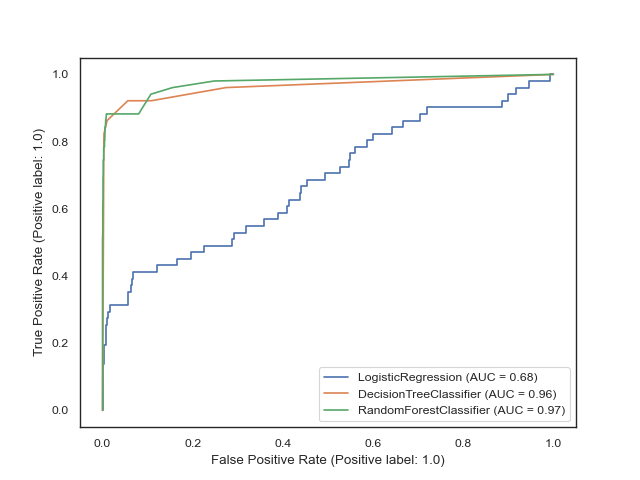
\includegraphics[width=.9\linewidth]{./data/roc.png}
	\caption{\label{fig:roc}ROC曲线与AUC值}
\end{figure}

\section{稳健性检验}
表 \ref{tab:Logitresult} 中作为财务指标的 \(Z\) 值显著。wind 数据库会直接提供 \(Z\) 值给投资者使用,其 \(Z\) 值的计算公式为
\begin{equation}
	\label{eq:1}
	Z=1.2X_1+1.4X_2+3.3X_3+0.6X_4+0.999X_5
\end{equation}
其中 \(X_1\)代表营运资本/总资产,\(X_2\)代表留存收益/总资产,\(X_3\)代表息税前利润/总资产:以上变量及 \(X_5\) 均可以直接获得一致的数据;\(X_4\)代表总市值/负债总计,而当企业非上市,总市值数据不可得时,则使用股东权益代替。

式 \ref{eq:1} 中的 \(X_{5}\) 包括了营业收入/总资产,和主营业务收入回归元存在一定的相关性。可能模型中主营业务收入非常显著,因而导致 \(Z\) 值显著,而非 \(Z\) 值本身带有一定的经济学逻辑。为检验此种可能性,本文将计算 \(Z\) 值的元素展开。如果该可能性成立,则有假设:

\begin{hyp}
	\label{hyp:1}
	展开 \(Z\) 值的回归结果 \(X_i\forall i\in [1,2,3,4] \) 应不显著,而仅仅是 \(X_5\) 显著。
\end{hyp}

\begin{center}
	\captionof{table}{稳健性检验结果\label{tab:robust}}
	\begin{tabular}{p{0.25\linewidth}p{0.2\linewidth}p{0.25\linewidth}p{0.2\linewidth}}
		\toprule
		\textbf{Dep. Variable:}   & default          & \textbf{  No. Observations:  } & 6447       \\
		\textbf{Model:}           & Probit           & \textbf{  Df Residuals:      } & 6414       \\
		\textbf{Method:}          & MLE              & \textbf{  Df Model:          } & 32         \\
		\textbf{Date:}            & Wed, 09 Mar 2022 & \textbf{  Pseudo R-squ.:     } & 0.7267     \\
		\textbf{Time:}            & 15:02:31         & \textbf{  Log-Likelihood:    } & -219.70    \\
		\textbf{converged:}       & True             & \textbf{  LL-Null:           } & -803.76    \\
		\textbf{Covariance Type:} & nonrobust        & \textbf{  LLR p-value:       } & 5.491e-225 \\
		\bottomrule
	\end{tabular}
	\begin{longtable}{p{0.18\linewidth}p{0.1\linewidth}p{0.1\linewidth}p{0.1\linewidth}p{0.1\linewidth}p{0.12\linewidth}p{0.1\linewidth}}
		\midrule
		                 & \textbf{coef} & \textbf{std err} & \textbf{z} & \textbf{P$> |$z$|$} & \textbf{[0.025} & \textbf{0.975]} \\
		\textbf{const}          & -3.8725       & 1.252            & -3.092     & 0.002               & -6.327          & -1.418          \\
		\textbf{评级\_A以上}    & -0.0382       & 0.318            & -0.120     & 0.904               & -0.661          & 0.585           \\
		\textbf{评级\_B}        & 1.4849        & 0.187            & 7.938      & 0.000               & 1.118           & 1.852           \\
		\textbf{评级\_C}        & 3.6740        & 0.228            & 16.102     & 0.000               & 3.227           & 4.121           \\
		\textbf{国有企业}       & -1.6422       & 0.398            & -4.128     & 0.000               & -2.422          & -0.862          \\
		\textbf{外资企业}       & -1.1744       & 0.467            & -2.514     & 0.012               & -2.090          & -0.259          \\
		\textbf{民营企业}       & -0.7078       & 0.385            & -1.839     & 0.066               & -1.462          & 0.046           \\
		\textbf{集体企业}       & -1.2313       & 0.534            & -2.307     & 0.021               & -2.277          & -0.185          \\
		\textbf{上市企业}       & -0.1945       & 0.192            & -1.014     & 0.310               & -0.570          & 0.181           \\
		\textbf{持有基金占比}   & -0.0783       & 0.080            & -0.973     & 0.331               & -0.236          & 0.079           \\
		\textbf{大股东持股比例} & -0.0013       & 0.003            & -0.508     & 0.611               & -0.006          & 0.004           \\
		\textbf{应付账款(万元)} & 1.409e-12     & 2.48e-12         & 0.567      & 0.570               & -3.46e-12       & 6.28e-12        \\
		\textbf{标准券折算率}   & -0.3647       & 0.651            & -0.560     & 0.575               & -1.640          & 0.911           \\
		\textbf{净资产(万元)}   & 9.314e-09     & 1.1e-08          & 0.847      & 0.397               & -1.22e-08       & 3.09e-08        \\
		\textbf{现金短债比}     & -0.1082       & 0.133            & -0.816     & 0.415               & -0.368          & 0.152           \\
		\textbf{流动性}         & -5.276e-11    & 6.63e-11         & -0.796     & 0.426               & -1.83e-10       & 7.72e-11        \\
		\textbf{政府支出/GDP}   & 1.2248        & 2.087            & 0.587      & 0.557               & -2.866          & 5.315           \\
		\textbf{SHIBOR}         & 0.3573        & 0.190            & 1.881      & 0.060               & -0.015          & 0.730           \\
		\textbf{波动率}         & 0.0341        & 0.016            & 2.135      & 0.033               & 0.003           & 0.065           \\
		\textbf{房地产政策}     & 0.7415        & 0.411            & 1.805      & 0.071               & -0.064          & 1.547           \\
		\textbf{X1}             & -0.0083       & 0.003            & -3.009     & 0.003               & -0.014          & -0.003          \\
		\textbf{X2}             & -0.0037       & 0.002            & -2.375     & 0.018               & -0.007          & -0.001          \\
		\textbf{X3}             & -0.0062       & 0.004            & -1.638     & 0.101               & -0.014          & 0.001           \\
		\textbf{X4}             & -0.0064       & 0.002            & -3.917     & 0.000               & -0.010          & -0.003          \\
		\textbf{X5}             & 0.0005        & 0.001            & 0.530      & 0.596               & -0.001          & 0.002           \\
		\bottomrule
	\end{longtable}
\end{center}

稳健性经验的部分结果如表
\ref{tab:robust}
所示,与表 \ref{tab:Logitresult} 相比基本一致,仅 SHIBOR 利率变为显著,且\(X_1\) 至 \(X_4\) 均显著,说明 \(Z\) 值中的其他成分均具有一定的预测能力,而非只是受到主营收入的影响导致显著,假设 H\ref{hyp:1}不成立。

事实上,\(Z\) 值反应了公司的变现能力、获利能力和财务结构,因而 Altman 使用其来对企业的运行状况进行分析。
公司的变现能力高意味着短期可以依靠出售资产回笼流动资金,避免流动性危机。典型的反例是土储集中在城郊地区的提前于行业倒下的泰禾地产,暴雷之后低价甩卖资产进一步恶化财务状况引发更多违约。
避免掏空式分红,利用留存收益和持续的利润增厚资本,可以使公司获得较强的抵御风险能力。譬如丹东港,高额分红导致资金短缺,资金缺口依靠债务回补,在融资审核趋严、实控人套现离场后留给当地违约的烂摊子。
公司的债券可以看作是卖出看跌期权,公司股权价值占比相对高,意味着公司价值距离行权价越远,KMV 等模型的违约距离也就越远,公司违约可能性相对较低。当然利用股权和债权融资都是适当的,公司不可过度偏废。综上 Z 值是一个很好的预测违约的指标。

%!TEX root = ../thesis.tex
\chapter{结论和展望}

2021 年以来,中资高收益债走入了至暗时刻,甚至对中国宏观经济造成了一定的影响。
部分过去曾经名誉较好的发行人走向了违约,有些企业官宣躺平寄希望于逃废债,一些边缘的企业也被艰难的融资环境挤向了违约,以至于发行人选择展期而不是全部甩给财务顾问重组都成了对投资人还算友好的债务处理方式。但更多的处于风暴中的企业仍在苦苦支撑不躺平,恪守信用不违约,努力产生现金流维持运转。

样本期内,我国经济形势总体是持续增长向好的。未来经济增速逐步放缓、经济发展不确定性增加的背景下,城投债如果违约亦将是打破预期的大冲击事件,也会对信用债市场造成冲击,影响非常多的实体企业,甚至于使本不该倒下的企业倒掉,影响无数普通人的生活。当前压垮这些企业的最重要的那根稻草,对避免未来相似的场景重新发生,也有一定的借鉴意义。

违约是且应当是经济中的正常现象,没有什么“大而不能倒”。然则前事不忘,后事之师。企业是经济中的细胞,如何避免某些单个的细胞坏死影响更多具有强大韧性的细胞,本文提出了一些显著性较高的指标。我们可以看到,就目前而言,企业保持健康的财务状况,适当适时扩大主营业务,维持一定的营运资本和息税前利润率,减少高分红竭泽而渔以增厚企业收益,规避高杠杆,提升资产周转率和利用率,这些都是是可以显著降低违约概率的措施,并且也都是企业正常健康发展的应有之义。政府应当保持稳健的政策,提供稳定的政策预期和融资环境,引导产业发展时不应过度扶持、只依赖补贴。在这个大变革的时代,虽然经济发展的前路艰险道阻且长,但只要少数企业的违约不发展成系统性风险,我们仍能对金融市场的稳定和发展保持信心。

\appendix
\printbibliography[heading = bibintoc]
% %!TEX root = ../thesis.tex
% Copyright (c) 2014,2016 Casper Ti. Vector
% Public domain.

\chapter{附件}

% vim:ts=4:sw=4

\backmatter
%!TEX root = ../thesis.tex
\chapter{致谢}

%!TEX root = ../thesis.tex
% Copyright (c) 2008-2009 solvethis
% Copyright (c) 2010-2017,2021 Casper Ti. Vector
% Copyright (c) 2021 Kurapica
% All rights reserved.
%
% Redistribution and use in source and binary forms, with or without
% modification, are permitted provided that the following conditions are
% met:
%
% * Redistributions of source code must retain the above copyright notice,
%   this list of conditions and the following disclaimer.
% * Redistributions in binary form must reproduce the above copyright
%   notice, this list of conditions and the following disclaimer in the
%   documentation and/or other materials provided with the distribution.
% * Neither the name of Peking University nor the names of its contributors
%   may be used to endorse or promote products derived from this software
%   without specific prior written permission.
%
% THIS SOFTWARE IS PROVIDED BY THE COPYRIGHT HOLDERS AND CONTRIBUTORS "AS
% IS" AND ANY EXPRESS OR IMPLIED WARRANTIES, INCLUDING, BUT NOT LIMITED TO,
% THE IMPLIED WARRANTIES OF MERCHANTABILITY AND FITNESS FOR A PARTICULAR
% PURPOSE ARE DISCLAIMED. IN NO EVENT SHALL THE COPYRIGHT HOLDER OR
% CONTRIBUTORS BE LIABLE FOR ANY DIRECT, INDIRECT, INCIDENTAL, SPECIAL,
% EXEMPLARY, OR CONSEQUENTIAL DAMAGES (INCLUDING, BUT NOT LIMITED TO,
% PROCUREMENT OF SUBSTITUTE GOODS OR SERVICES; LOSS OF USE, DATA, OR
% PROFITS; OR BUSINESS INTERRUPTION) HOWEVER CAUSED AND ON ANY THEORY OF
% LIABILITY, WHETHER IN CONTRACT, STRICT LIABILITY, OR TORT (INCLUDING
% NEGLIGENCE OR OTHERWISE) ARISING IN ANY WAY OUT OF THE USE OF THIS
% SOFTWARE, EVEN IF ADVISED OF THE POSSIBILITY OF SUCH DAMAGE.

{
	\ctexset{section = {
		format+ = {\centering}, beforeskip = {40bp}, afterskip = {15bp}
	}}
	\specialchap{北京大学学位论文原创性声明和使用授权说明}

	% 学校书面要求本页面不要页码,但在给出的 Word 模版中又有页码。
	% 此处以学校书面要求为准。
	\thispagestyle{empty}
	\mbox{}\vspace*{-3em}
	\section*{原创性声明}

	本人郑重声明:
	所呈交的学位论文,是本人在导师的指导下,独立进行研究工作所取得的成果。
	除文中已经注明引用的内容外,
	本论文不含任何其他个人或集体已经发表或撰写过的作品或成果。
	对本文的研究做出重要贡献的个人和集体,均已在文中以明确方式标明。
	本声明的法律结果由本人承担。
	\vskip 1em
	\rightline{%
		论文作者签名:\hspace{5em}%
		日期:\hspace{2em}年\hspace{2em}月\hspace{2em}日%
	}

	\section*{%
		学位论文使用授权说明\\[-0.33em]
		\textmd{\zihao{5}(必须装订在提交学校图书馆的印刷本)}%
	}

	本人完全了解北京大学关于收集、保存、使用学位论文的规定,即:
	\begin{itemize}
		\item 按照学校要求提交学位论文的印刷本和电子版本;
		\item 学校有权保存学位论文的印刷本和电子版,
			并提供目录检索与阅览服务,在校园网上提供服务;
		\item 学校可以采用影印、缩印、数字化或其它复制手段保存论文;
		\item 因某种特殊原因须要延迟发布学位论文电子版,
			授权学校 $\Box$\nobreakspace{}一年 /
			$\Box$\nobreakspace{}两年 /
			$\Box$\nobreakspace{}三年以后,在校园网上全文发布。
	\end{itemize}
	\centerline{(保密论文在解密后遵守此规定)}
	\vskip 1em
	\rightline{%
		论文作者签名:\hspace{5em}导师签名:\hspace{5em}%
		日期:\hspace{2em}年\hspace{2em}月\hspace{2em}日%
	}

	% 若须排版二维码,请将二维码图片重命名为“barcode”,
	% 转为合适的图片格式,并放在当前目录下,然后去掉下面 2 行的注释。
	%\vfill\noindent
	%\includegraphics[height = 5em]{barcode}
}

% vim:ts=4:sw=4

\end{document}
